\chapter{Design}
    This chapter aims to first extend the concepts of $\Delta$QSD, giving more insights into how the systems need to be instrumented to correctly work together, and how the different parts need to be integrated to interact together.
    \begin{itemize}
        \item We first provide concepts of probes, we extend the $\Delta$QSD notion of failure and describe how time series will work in our oscilloscope, this part is crucial to understand how the measurements are done in real time.
        \item We then split the design of the oscilloscope in two. First explaining the Erlang side, where the system to be tested is. Secondly, we explain the C++ side. Both chapters explain how probes can be inserted and made to work together.
        \item Lastly, we provide high level concepts of triggers and execution windows, the key elements of the oscilloscope. 
    \end{itemize}

    Before delving deeper into the chapter, we present the global system design diagram.

    \begin{figure}[H]
        \begin{center}
            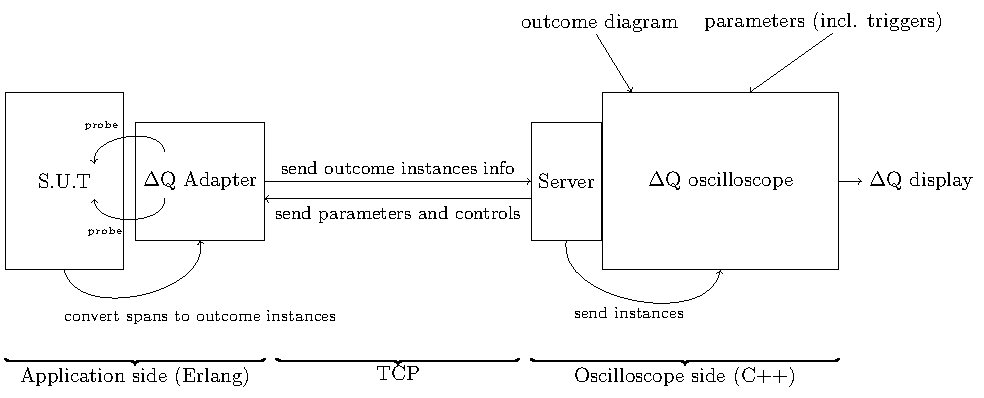
\includegraphics[width=\textwidth]{tikz/sut-stub-osc.pdf}
        \end{center}
        \caption{Global system design diagram. The two sides communicate via TCP sockets to share information about outcome instances and probe parameters.}
    \end{figure}

    We can recognise two distinct parts:
    \begin{itemize}
        \item The application side, where the Erlang system under test is. Consequently, it's where the $\Delta$Q adapter will be, which performs the translation of spans to outcome instances thanks to probes.
        \item The oscilloscope side, where the $\Delta$Q oscilloscope receives information from the adapter attached to the system under test to display graphs, define outcome diagrams and set parameters for probes.
    \end{itemize}


    \section{Measurement concepts}
    \subsection{Probes}

A system instrumented with OpenTelemetry has spans and traces to observe the execution of an operation \cite{otel-t}. The same level of observability must be assured in the oscilloscope, this is why we provide the concept of probes, which, like spans, follow an execution from start to end. \textbf{Note} that a definition of probes has already been introduced in a previous article relating to $\Delta$QSD \cite{dq-br}, but the concept we present here is not the same.

To observe a system, we must put probes in it. For each outcome of interest, a probe (observation point) is attached to measure the delay of the outcome, like one would in a true oscilloscope \cite{post}.

Consider \cref{fig:probes} below. A probe is attached at every component (for example, a database \cite{dq-tut}) to measure their $\Delta$Qs ($p_2, p_3$). Another probe ($p_1$) is inserted at the beginning and end of the system to measure the global execution delay. Thanks to this probe, the user can observe the $\Delta$Q \textit{``observed at $p_1$''}, which is the $\Delta$Q which was calculated from the data received by inserting probe $p_1$. The \textit{$\Delta$Q ``calculated at $p_1$''} is the resulting $\Delta$Q from the convolution of the observed $\Delta$Qs at $c_2$ and $c_3$. \\
Probe $p_1$ is the equivalent of a ``root/parent span'' which observe the whole execution of $c_1, c_2$, while $p_2$ and $p_3$ are child spans which represent single instances of execution.

    \begin{figure}[H]
        \begin{center}
            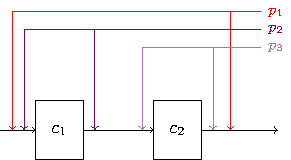
\includegraphics[scale=1.8]{tikz/probes.pdf}
        \end{center}
        \caption{Probes inserted in a component diagram. In an application instrumented with OpenTelemetry, $p_1$ could be considered the root span, $c_1$ and $c_2$ its children spans sharing a causal link.}
        \label{fig:probes}
    \end{figure}




    \subsection{Extending failure}
   Recall the definition of failure: \textit{``an input message $m_{in}$ that has no output message $m_{out}$''} \cite{art}. In the previous section \ref{fig:otel_dmax}, we also introduced the notion of a maximum delay. 

   By extending the notion of failure to include $dMax$, we can know right away when execution is straying away from engineer defined behaviour, avoiding having to wait until the execution is done. In $\Delta$QSD, an execution may as well take 10 or 15 seconds, but if the delay of execution is $> dMax$, we consider that \textbf{failed} right away, we do not need to know the total execution time, the execution has already taken too much \cite{myo}. The full span will be exported regardless to monitoring tools which were set up by the user. 

   The user can observe both real time information with $\Delta$QSD notion of failure on the $\Delta$Q oscilloscope, and observe those spans in their monitoring tools if they wish.

The notion of failure is extended to the following definition:
        \begin{center}
            \textit{``An input message $m_{in}$ that has no output message $m_{out}$ after $dMax$''} 
        \end{center}
    We can leverage this new definition to observe the system and the $\Delta$Qs in real time.


    \subsection{Time series of outcome instances}
    Consider a probe $p$ with two distinct sets of events, the starting set of events $s$ and ending set of event $e$. The outcome instance of a message $m_s \rightarrow m_e$ contains:
    \begin{itemize}
        \item The probe's $p$ name
        \item The start time $t_s$
        \item The end time $t_e$
        \item Its status 
        \item Its elapsed time of execution
    \end{itemize}
    The instance has three possible statuses: \texttt{success, timeout, failure}, it can thus be broken down in the representations, based on its status:
    \begin{itemize}
        \item \textbf{($t_s$,$t_e$)}: This representation indicates that the execution was successful (t $<$ $dMax$). 
        \item \textbf{($t_s, \mathcal{T}$)}: This representation indicates that the execution has timed out (t $>$ $dMax$). The end time and elapsed time is equal to $t_s + \text{timeout}$ 
        \item \textbf{($t_s, \mathcal{F}$)}: This representation indicates the execution has failed given a user defined requirement (i.e. a dropped message given buffer overload in a queue system). It must not be confused with a program failure (crash), if a program crashes during the execution of event $e$, it will time out since the adapter will not receive an end message.
    \end{itemize}
    The \textbf{time series} of a probe is the sequence of $n$ outcome instances and can then be easily modeled by $\Delta$Q.

    \paragraph{What can be considered a failed execution?} Imagine a queue with a buffer: the buffer queue being full and dropping incoming messages can be modeled as a failure.

    More generally, the choice of what is considered a failed execution is left up to the user who is handling the spans and is program-dependent. Exceptions or errors can be kinds of failure. 

    On another note, the way of handling errored spans in OpenTelemetry can differ from user to user, so the adapter will not handle ending and setting statuses for "failed" spans. \cite{otel-err}
   
   In any case, by the new definition of failure, \textbf{timed out and failed will both be considered as a failure} in the calculation of a $\Delta$Q.

    \section{Application side} 
    \subsection{System under test} The system under test \textbf{(S.U.T)} is the Erlang system the engineer wishes to observe (\cref{fig:sys_diag}). It ideally is a system which already is instrumented with OpenTelemetry. The ideal system where $\Delta$QSD is more useful is a system that executes many independent instances of the same action \cite{dq-tut}. 
    
    \subsection{$\Delta$Q Adapter} 
    The $\Delta$Q adapter is the \texttt{dqsd\_otel} Erlang interface \cite{wrapper}. It starts and ends OpenTelemetry spans and translates them to outcome instances which are useful for the oscilloscope. This can be done thanks to probes being attached to the system under test, like an oscilloscope would. The outcome instances end normally like OpenTelemetry spans or, additionally, can timeout after a custom timeout ($dMax$), and fail, \textit{according to user's definition of failure}. 
    
    Handling of OpenTelemetry spans which goes beyond starting and ending them is delegated to the user, who may wish to do further operations with their spans. 
    The adapter is called from the system under test and communicates outcome instances data to the oscilloscope via TCP sockets. 
    
    The adapter can receive messages from the oscilloscope, the messages are about updating probe's $dMax$ or starting and stopping the sending of data to the oscilloscope.
    \subsection{Inserting probes in Erlang - From spans to outcome instances}
        OpenTelemetry spans are useful to carry context, attributes and baggage in a program \cite{otel-dt}. The plethora of attributes they have is nevertheless too much for the oscilloscope. 
        To get the equivalent of spans for the oscilloscope, the adapter needs to be called at the starting events of a probe to start an instance of a probe, and at the ending events to end the outcome instance. The name given with \texttt{``start\_span/with\_span''} is the name of the probe. The PID which is returned by starting a span must be carried throughout the whole execution, and used when ending spans to create the correlation between a probe and an outcome instance.
\begin{figure}[H]
\centering
   \begin{minted}{erlang}
        % Start the outcome instance of probe. The call to dqsd_otel starts an OpenTelemetry span, as it contains a call to ?start_span(Name)
        {ProbeCtx, ProbePid} = dqsd_otel:start_span(<<"probe">>),  

        % Start and fail span directly
        {WorkerCtx, WorkerPid} = dqsd_otel:start_span(<<"worker_1">>),   
        dqsd_otel:fail_span(WorkerPid),
        %Here, you would need to end the span manually with ?end_span

        %Example of with_span, the call to OpenTelemetry ?with_span is inside the adapter function, the function fun() -> ok end is executed inside dqsd_otel.
        dqsd_otel:with_span(<<"worker_2">>, fun() -> ok end), 
        %End the outcome instance of probe. This ends the OpenTelemetry span aswell. If the outcome instance has already timed out (the time from start_span to end_span > dMax), the oscilloscope receives no message where the status is successful. Otherwise, this sends a message with startTime, endTime, the name "probe" and success status.
        dqsd_otel:end_span(ProbeCtx, ProbePid),
        \end{minted}
\caption{Example usage of the adapter}\label{code:adapter}
\end{figure}
    Further details about the implementation of the adapter are explained in Chapter 5. A user guide on how to include the adapter in your project and how to instrument a program is found in the appendix (\cref{app:instr_app}). 
  
    \section{Oscilloscope side}
    \subsection{Server} The server is responsible for receiving the messages containing the outcome instances from the adapter. The server forwards the instances to the oscilloscope.
    
    \subsection{$\Delta$Q Oscilloscope} The oscilloscope is a C++ graphical application which implements a dashboard to observe $\Delta$Qs of probes inserted in the system under test \cite{osc-g}. It receives the instances corresponding to probes from the server and adds them to the time series of the probes whose instance is being received. 
    The oscilloscope has a graphical interface which allows the user to create an outcome diagram of the system under test, display real time graphs which show detail about the execution of the system and allow the user to set parameters for probes. It can also display snapshots of the system as if it was frozen in time.

    \subsection{Inserting probes in the oscilloscope}
        Probes are automatically inserted in the oscilloscope when creating outcome diagrams. They are inserted on the outcomes observables, operators observables and to the sub-outcome diagrams observables (probes that observe the causal links of multiple outcomes/operators), we will see later on how they can be defined and how an outcome diagram can be created. \\
    The names that are given to outcome, operators and sub-outcome diagrams are the names of the probes that observe them. Giving these probes a name allows the oscilloscope to match the outcome instances to the probes' time series.

        In the system below, which is equal to the one defined above, probes are automatically attached to outcomes $o_1, o_2$. The user who wants to observe the result of the sequential composition can insert probes at the start and end of the routine. 
    
        \begin{figure}[H]
            \begin{center}
                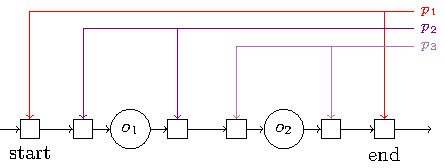
\includegraphics[scale=1.3]{tikz/probe_1.pdf}
            \end{center}
            \label{fig:probes_o}
            \caption{Probes inserted in the outcome diagram of the previous component diagram in \cref{fig:probes}.}
        \end{figure}
       
    The \textbf{observables} are an abstract representation of events. Consider the previous code snippet \cref{code:adapter}: the $start$ event of ``probe'' and worker$_1$'s start event are subsequent instructions. The probe's start event is practically the same as worker$_1$'s start event, indeed, they could be overlapped in the graph above. We nevertheless show the distinction to show that probe and worker$_1$ need to be started differently in Erlang as the information they carry is about two distinct instances. Furthermore, this difference is remarked in the definition of outcome diagrams, for which we provide a syntax in the following chapter. 
    
    As for operators, probes are automatically attached to the components inside them and to the start event and end events of the operators (its observables). 

       \begin{figure}[H]
           \begin{center}
                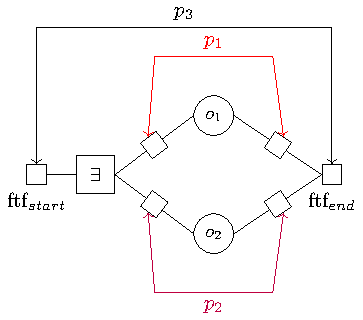
\includegraphics[scale = 1.3]{tikz/probe_2.pdf}
            \end{center}
            \label{fig:probes_op}
            \caption{Probes inserted into an operator.}
       \end{figure}
    
    The \textbf{observed $\Delta$Q} for the first-to-finish operator is the $\Delta$Q for the observables (\textbf{start}, \textbf{end}). The \textbf{calculated $\Delta$Q} is the $\Delta$Q which is the result of the first-to-finish operator being applied on $o_1, o_2$.

        



    

    \section{Triggers}
    Much like an oscilloscope that has a trigger mechanism to capture periodic signals or investigate a transient event \cite{osc-t}, the \textit{$\Delta$Q oscilloscope} has a similar mechanism that can recognise when an observed $\Delta$Q violates certain conditions regarding required behaviour and record snapshots of the system.

    Each time an observed $\Delta$Q is calculated, it is checked against the requirements set by the user. If these requirements are not met, a trigger is fired and a snapshot of the system is saved to be shown to the user. 
    
    \subsection{Snapshot}
    A snapshot of the system gives insights into the system before and after a trigger was fired. It gives the user a still of the system, as if it was frozen in time. All the $\Delta$Qs which are calculated during the system's execution are stored away. Then, if no trigger is fired, older $\Delta$Qs are removed. Otherwise, the oscilloscope keeps recording $\Delta$Qs without removing older ones, to allow the user to look at the state of the system before and after the trigger.
    

    \section{Sliding execution windows}

    There are two important windows that we consider in our oscilloscope, the \textit{sampling window} and the \textit{polling window}.

    \subsection{Sampling window}
    Suppose we are at time $t$, the observed (and calculated, if applicable) $\Delta$Qs at time $t$ we will display are the $\Delta$Qs obtained from the outcome instances who ended within a sampling window in the \textbf{window of time $(t-1)_{l}$ - $(t-1)_u$}, with $t-1$ equal to $t - x$, and $x$ the sampling rate. The sampling rate is how often $\Delta$Qs are calculated. \\
    This is to account for various overheads that need to be taken into consideration. They could be network overhead, the adapter overhead, C++ latency \dots Imagine multiple outcome instances that are ended at a time slightly lower but close to t, and due to the overheads the messages arrive at a time slightly higher but close to t, the outcome instance would not be taken into consideration for the calculation of a $\Delta$Q.
    
    \begin{figure}[H]
        \begin{center}
            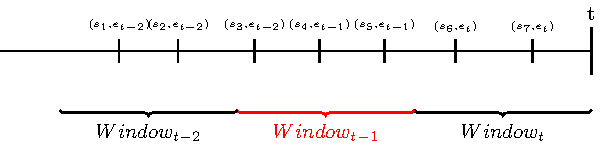
\includegraphics{tikz/window.pdf}
        \end{center}
    \end{figure}
    
    The sampling window then advances every $x$ seconds, setting the new window: 
    \begin{center}
        From: $(t-1)_l$, $(t-1)_u$ $\xrightarrow{t + 1}$ $t_l, t_u$. \\
        Where: $t_l = (t-1)_u$ and $t_u = (t-1)_u + x$ 
    \end{center}
    
    The $\Delta$Qs which are observed and calculated in a sampling window are not precise, this is why we need to introduce the polling window.

    \subsection{Polling window (Observing multiple $\Delta$Qs over a time interval)}
        The polling window is the window of $\Delta$Qs which are stored to keep a snapshot of the system over time and over which confidence bounds are calculated. The polling window serves to improve the precision of the $\Delta$Q measurement.
        
        Suppose we are at time $t = 0$, the polling window will have 0 $\Delta$Qs. As the sampling window advances, more $\Delta$Qs are sampled, which in turn are added to the snapshot and to the confidence bounds.

        The limit of $\Delta$Qs for a polling window (subsequently snapshots and confidence bounds) is 30 $\Delta$Qs. At $t= 31$, the older $\Delta$Qs will be removed from the polling window and in turn from the snapshots and confidence bounds. Newer sampled $\Delta$Qs will be added, keeping the limit of $\Delta$Qs in a polling window to 30.


